% !TeX program = pdflatex
% !TeX encoding = UTF-8
\documentclass[12pt,aspectratio=169]{beamer}

% Standard Beamer presentation.
% The slides intentionally use Beamer's ordinary title bars, bullets, blocks,
% and footline. The PPTX files are used as content references, not design templates.
\usetheme{Madrid}
\useinnertheme{rounded}
\usefonttheme{professionalfonts}

\usepackage{kotex}
\usepackage[scaled=0.94]{helvet}
\renewcommand{\familydefault}{\sfdefault}
\usepackage{graphicx}
\usepackage{xurl}
\usepackage{tabularx}
\usepackage{array}
\usepackage{amsmath,amssymb}

\graphicspath{{figures/}{figures/timetable/}}
\urlstyle{same}

\definecolor{POSTECHRed}{RGB}{200,16,46}
\definecolor{POSTECHDark}{RGB}{25,25,25}

\setbeamercolor{normal text}{fg=black,bg=white}
\setbeamercolor{structure}{fg=POSTECHRed}
\setbeamercolor{alerted text}{fg=POSTECHRed}
\setbeamercolor{palette primary}{fg=white,bg=POSTECHRed}
\setbeamercolor{palette secondary}{fg=white,bg=POSTECHDark}
\setbeamercolor{palette tertiary}{fg=white,bg=POSTECHRed}
\setbeamercolor{palette quaternary}{fg=white,bg=POSTECHDark}
\setbeamercolor{frametitle}{fg=white,bg=POSTECHRed}
\setbeamercolor{title}{fg=white,bg=POSTECHRed}
\setbeamercolor{titlelike}{fg=white,bg=POSTECHRed}
\setbeamercolor{block title}{fg=white,bg=POSTECHRed}
\setbeamercolor{block body}{fg=black,bg=black!5}
\setbeamercolor{item projected}{fg=white,bg=POSTECHRed}
\setbeamercolor{subitem projected}{fg=white,bg=POSTECHRed}

\setbeamertemplate{navigation symbols}{}
\setbeamertemplate{items}[circle]
\setlength{\parskip}{0.22em}
\setbeamerfont{itemize/enumerate body}{size=\normalsize}
\setbeamerfont{itemize/enumerate subbody}{size=\small}
\setbeamerfont{block body}{size=\normalsize}

\newenvironment{mainitemize}{\begin{itemize}\setlength{\itemsep}{0.72em}}{\end{itemize}}
\newenvironment{subitemize}{\begin{itemize}\setlength{\itemsep}{0.22em}}{\end{itemize}}
\newcommand{\smallurl}[1]{{\scriptsize\url{#1}}}

% Three-part standard Beamer footline.
% Keeps the ordinary Madrid layout but separates speaker, school, and department.
\makeatletter
\setbeamertemplate{footline}{%
  \leavevmode%
  \hbox{%
    \begin{beamercolorbox}[wd=.33\paperwidth,ht=2.25ex,dp=1ex,center]{author in head/foot}%
      \usebeamerfont{author in head/foot}Jungwoo Kim
    \end{beamercolorbox}%
    \begin{beamercolorbox}[wd=.34\paperwidth,ht=2.25ex,dp=1ex,center]{title in head/foot}%
      \usebeamerfont{title in head/foot}POSTECH
    \end{beamercolorbox}%
    \begin{beamercolorbox}[wd=.33\paperwidth,ht=2.25ex,dp=1ex,right]{date in head/foot}%
      \usebeamerfont{date in head/foot}Department of Mathematics\hspace*{1.5em}\insertframenumber{} / \inserttotalframenumber\hspace*{2ex}
    \end{beamercolorbox}%
  }%
  \vskip0pt%
}
\makeatother


\title[Department of Mathematics]{Department of Mathematics, POSTECH}
\subtitle{포항공과대학교 수학과}
\author[Jungwoo Kim]{Jungwoo Kim 김정우}
\institute[POSTECH]{@jkpxt14\\jkpxt14@postech.ac.kr}
\date{}

\begin{document}

\begin{frame}
  \titlepage
\end{frame}

\begin{frame}{Self-Introduction}
\begin{mainitemize}
  \item 서울고등학교 77기 졸업
    \begin{subitemize}
      \item 과학중점반
      \item 수학부 Fractal 부장
    \end{subitemize}
  \item 포항공과대학교 수학과 25학번 재학
    \begin{subitemize}
      \item 무은재학부 입학, 수학과 선택 \& 컴퓨터공학과 복수전공
      \item 포항공과대학교 방송국 PBS
      \item 2026 포스텍-카이스트 학생대제전 과학퀴즈 수학 대표 선수
    \end{subitemize}
\end{mainitemize}
\vspace{0.25em}
\smallurl{https://github.com/jkpxT14/POSTECH/tree/main/(POKA001)\%20Science\%20Quiz}
\end{frame}

\begin{frame}{Heads-up}
\begin{mainitemize}
  \item 본 발표는 이공계 관련 내용을 중점적으로 다룬다.
  \item 메디컬을 목표한다면 성적을 잘받는 것이 그 무엇보다 중요하다.
    \begin{subitemize}
      \item 전교 5등 이내를 목표로 하자!
    \end{subitemize}
\end{mainitemize}
\end{frame}

\begin{frame}{POSTECH}
\begin{mainitemize}
  \item 소수정예 \& 연구중심
  \item 전액 장학금
  \item 1000만원 바우처 지급
  \item 무료로 최신 아이패드, 에어팟 제공
  \item 1학년 때부터 교수님과의 연구가 가능하다.
\end{mainitemize}
\end{frame}

\begin{frame}{Residential College (RC)}
\begin{mainitemize}
  \item 1학년 때에는 전원이 기숙사 생활을 한다.
  \item 전국에서 가장 깔끔하고 현대적인 기숙사
  \item 분반 친구들과 수업도 같이 듣고, 기숙사에서도 함께한다.
\end{mainitemize}
\end{frame}

\begin{frame}{POSTECH-KAIST Science War}
\begin{mainitemize}
  \item 포스텍-카이스트 학생대제전, 줄여서 포카전
  \item 고연전과 비슷하다.
  \item 축구, 농구, 야구, 이스포츠(리그 오브 레전드), 과학퀴즈, 인공지능, 해킹
  \item 올해 포스텍 승리 예정!!
\end{mainitemize}
\end{frame}

\begin{frame}{Mueunjae School of Undergraduate Studies}
\begin{mainitemize}
  \item 무은재학부 (무전공, 자유전공)
  \item 2학년 2학기부터 특정 학과에 배정된다.
\end{mainitemize}
\begin{block}{2026 Department Application Results}
\small
수학과(13), 물리학과(25), 화학과(4), 생명과학과(14), 신소재공학과(37), 기계공학과(28), 산업경영공학과(20), 전자전기공학과(63), 컴퓨터공학과(42), 화학공학과(38), IT융합공학과(의공학과)(3) / 반도체공학과
\end{block}
\end{frame}

\begin{frame}{Curriculum}
\begin{columns}[T,totalwidth=\textwidth]
  \begin{column}{0.49\textwidth}
    \centering
    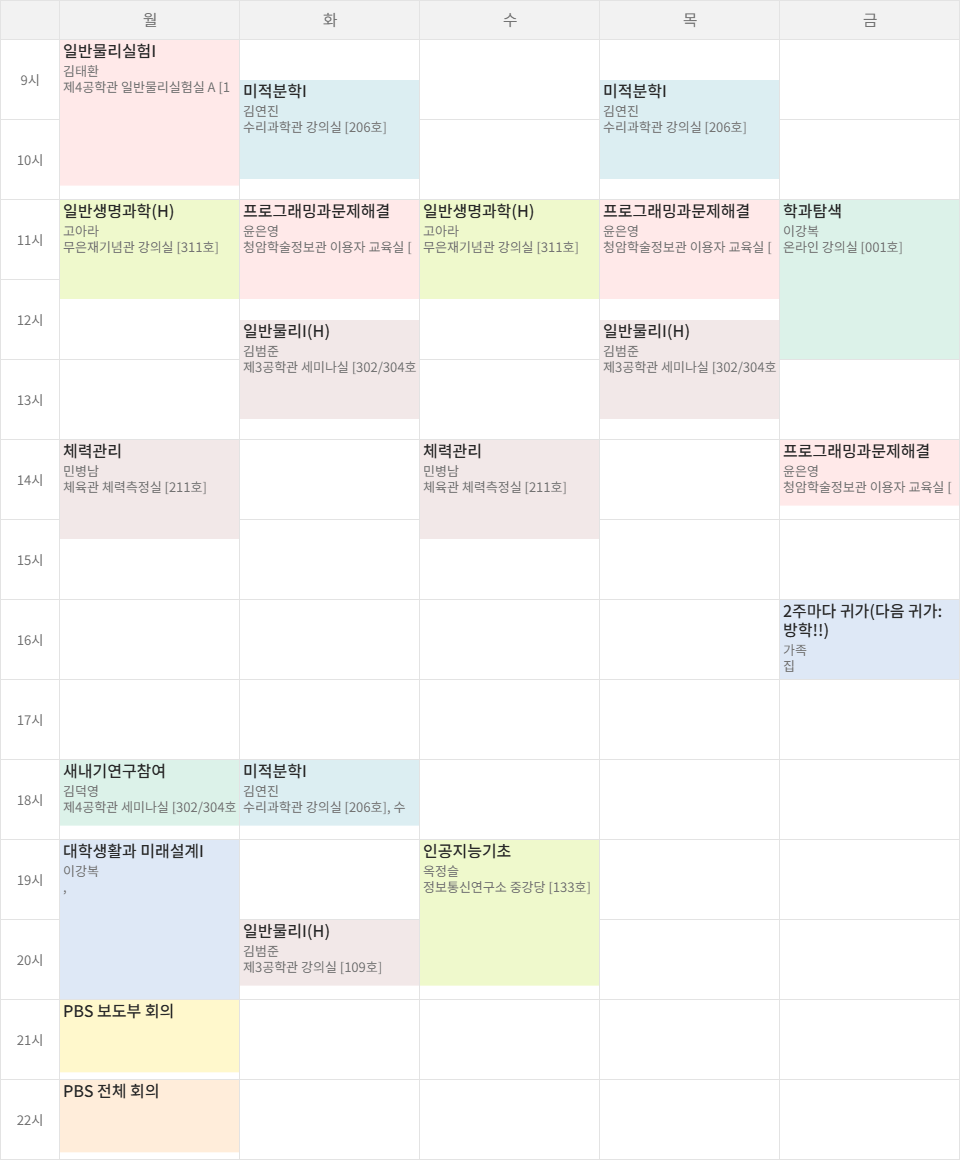
\includegraphics[height=0.72\textheight,width=\linewidth,keepaspectratio]{2025Spring.png}\\[-0.2em]
    {\small 2025 Spring}
  \end{column}
  \begin{column}{0.49\textwidth}
    \centering
    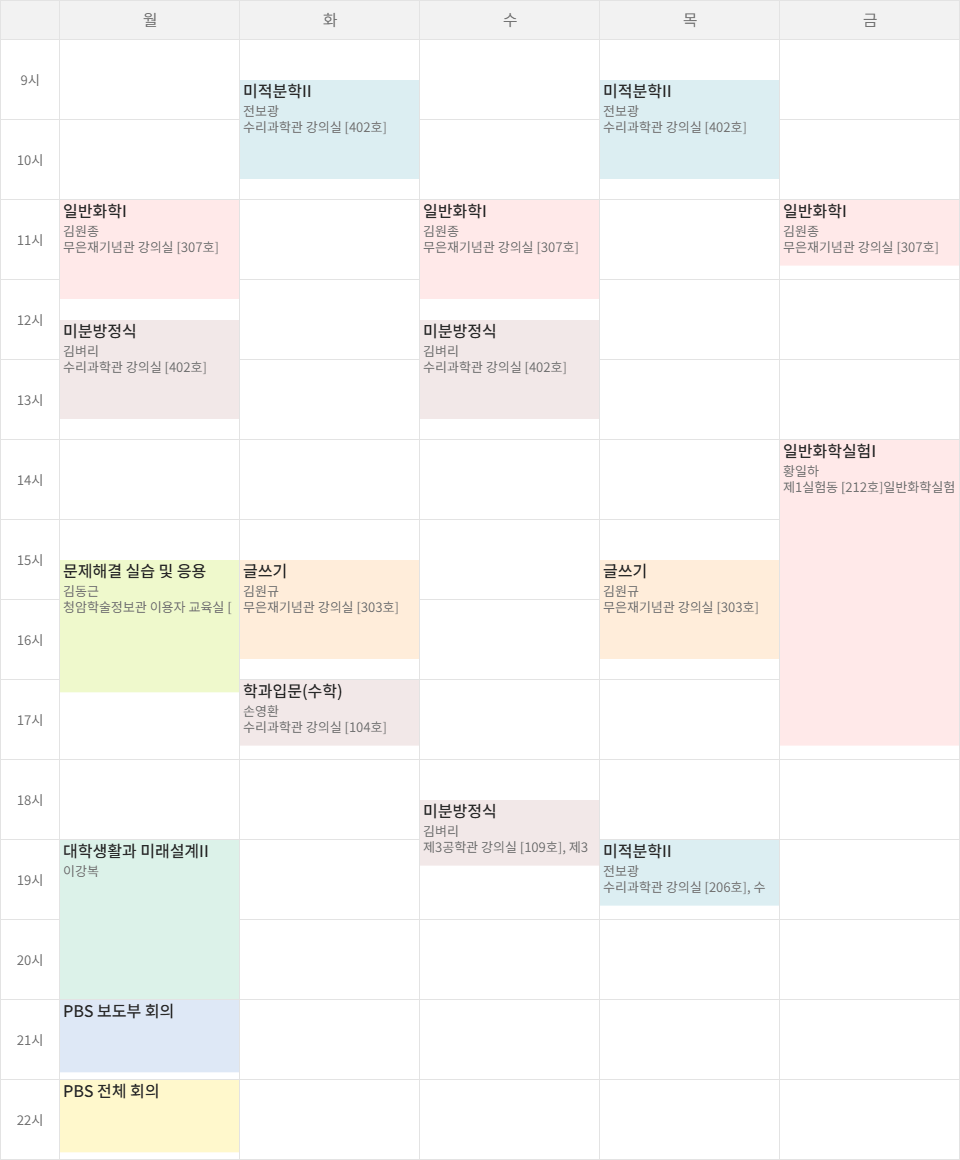
\includegraphics[height=0.72\textheight,width=\linewidth,keepaspectratio]{2025Fall.png}\\[-0.2em]
    {\small 2025 Fall}
  \end{column}
\end{columns}
\end{frame}

\begin{frame}{Department of Mathematics}
\vfill
\begin{center}
{\Large 수학을 공부하고 연구하는 학과}
\end{center}
\vfill
\end{frame}

\begin{frame}{University Math (vs High School Math)}
\begin{mainitemize}
  \item 고등학교 수학과는 다르다.
  \item 대학교 수학은 매우 추상적이다.
  \item 수학을 하나의 언어로서 받아들이는 감각이 중요하다.
  \item 수능 수학 문제 푸는 것이 재밌어서 수학과 진학을 고려 중이라면 공대를 가자.
  \item 한 문제를 깊게 고민하는 끈기가 중요하다.
  \item 단적인 예로 수능 수학은 30문제에 100분, 대학교 수학 시험은 10문제에 200분이 주어진다.
\end{mainitemize}
\end{frame}

\begin{frame}{CSAT, KMO, IMO, Putnam vs Research}
\begin{block}{Majoring in Mathematics}
수학을 ‘전공’한다는 것은, 답이 알려진 문제를 푼다는 것이 아니다.
\end{block}
\begin{block}{Research in Mathematics}
새로운 문제를 정의하고, 답이 없는 문제의 답을 유추하고, 엄밀한 증명을 적어나가고, 새로운 구조를 쌓아나가는 것이 수학에서의 ‘연구’이다.
\end{block}
\end{frame}

\begin{frame}{Artificial Intelligence in Mathematics}
\begin{block}{References}
{\scriptsize
\url{https://deepmind.google/blog/advanced-version-of-gemini-with-deep-think-officially-achieves-gold-medal-standard-at-the-international-mathematical-olympiad/}\par\medskip
\url{https://www.prezenceai.com/en/ainow/imo-2026-llms-pontuacao-perfeita-42-42-claude-fable-gpt-sol-kimi.html}
}
\end{block}
\end{frame}

\begin{frame}{The same goes for other fields}
\begin{mainitemize}
  \item 수학에서만 일어나고 있는 일이 아니다.
  \item 인공지능의 동향을 살피는 것이 중요하다.
  \item 인공지능을 배척하는 것은 시대에 뒤떨어지는 일이다.
  \item 인공지능에 잠식당하지 않고 주체성을 유지한 채 활용하자.
\end{mainitemize}
\end{frame}

\begin{frame}{Standard Curriculum}
\begin{mainitemize}
  \item 1학년: 미적분학I, 미적분학II, 응용선형대수, 미분방정식, 확률 및 통계
  \item 2학년: 집합론, 정수론, 현대대수학I, 해석학I, 응용복소함수론, 이산수학
  \item 3학년: 현대대수학II, 해석학II, 일반위상수학, 선형대수학
  \item 3, 4학년: 전공 마음껏 (대학원 개설 과목까지 수강 가능)
\end{mainitemize}
\end{frame}

\begin{frame}{My Curriculum (Major)}
\begin{columns}[T,totalwidth=\textwidth]
  \begin{column}{0.49\textwidth}
    \centering
    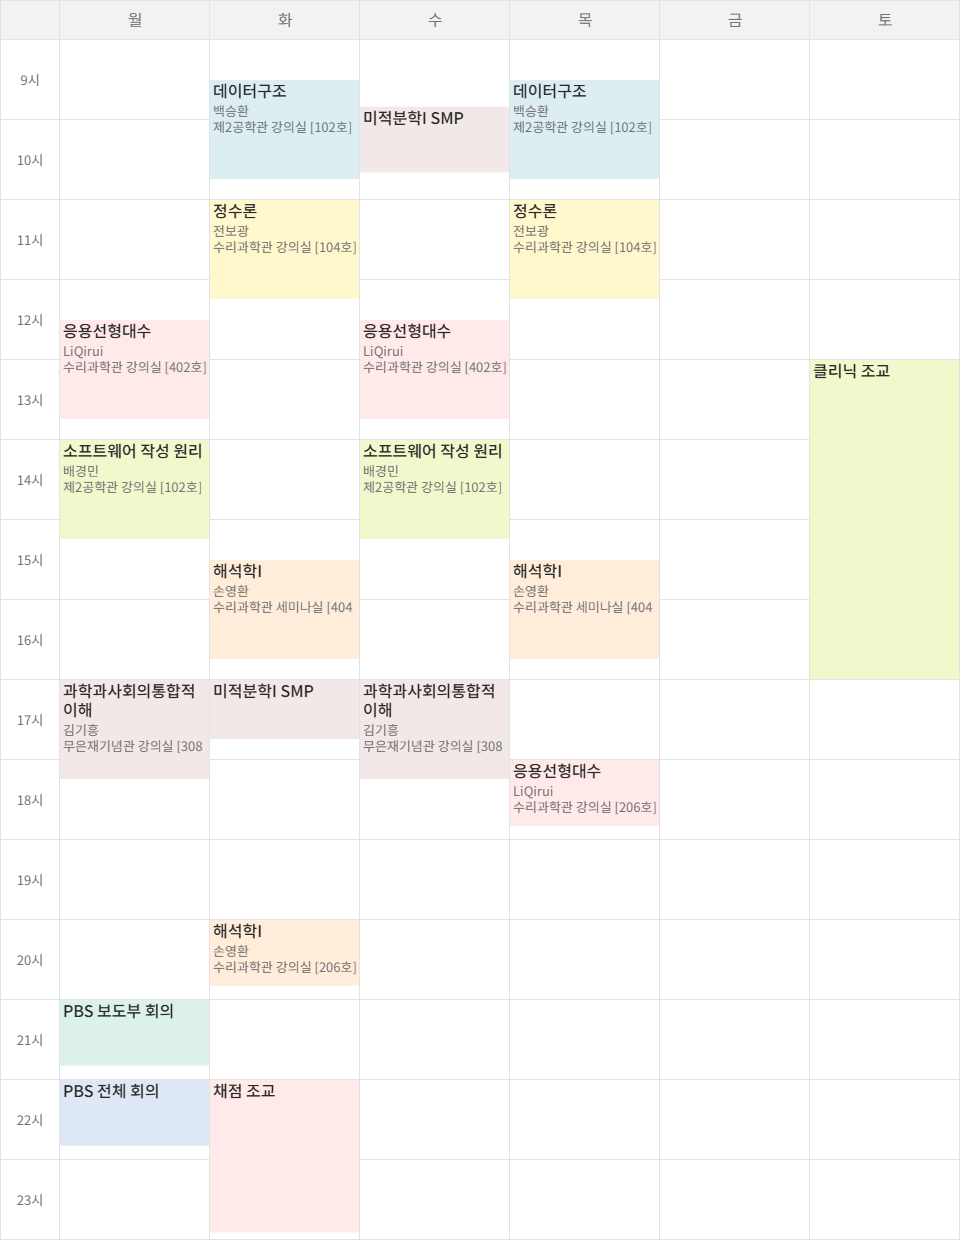
\includegraphics[height=0.72\textheight,width=\linewidth,keepaspectratio]{2026Spring.png}\\[-0.2em]
    {\small 2026 Spring}
  \end{column}
  \begin{column}{0.49\textwidth}
    \centering
    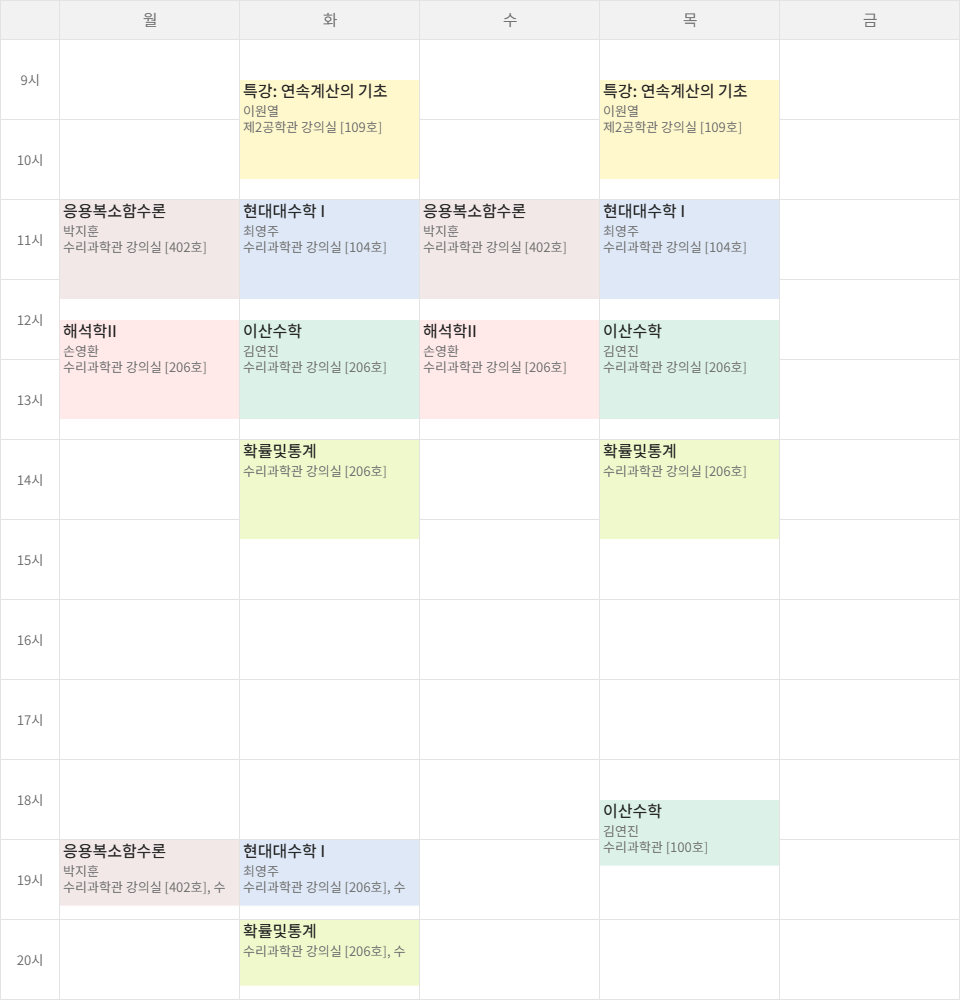
\includegraphics[height=0.72\textheight,width=\linewidth,keepaspectratio]{2026Fall.png}\\[-0.2em]
    {\small 2026 Fall}
  \end{column}
\end{columns}
\end{frame}

\begin{frame}{My Curriculum (General)}
\begin{columns}[T,totalwidth=\textwidth]
  \begin{column}{0.49\textwidth}
    \centering
    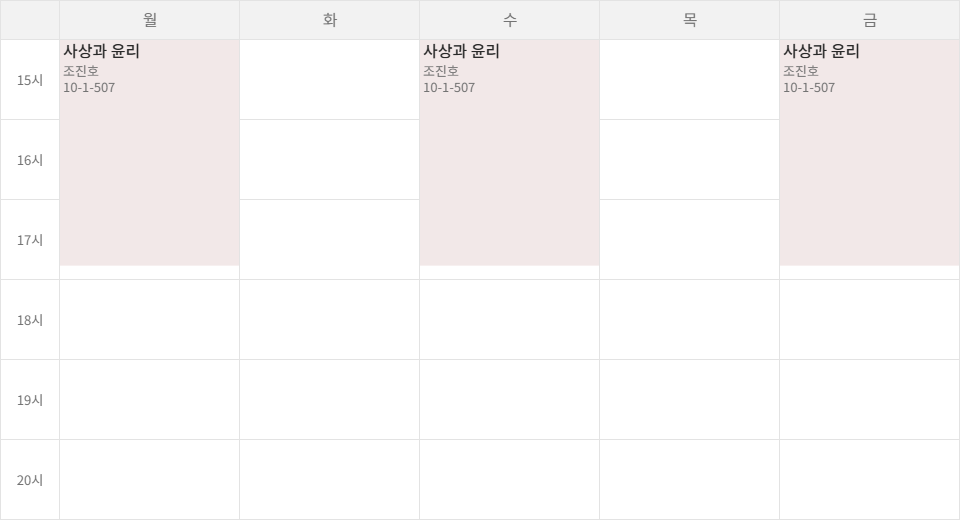
\includegraphics[height=0.72\textheight,width=\linewidth,keepaspectratio]{2025Summer.png}\\[-0.2em]
    {\small 2025 Summer}
  \end{column}
  \begin{column}{0.49\textwidth}
    \centering
    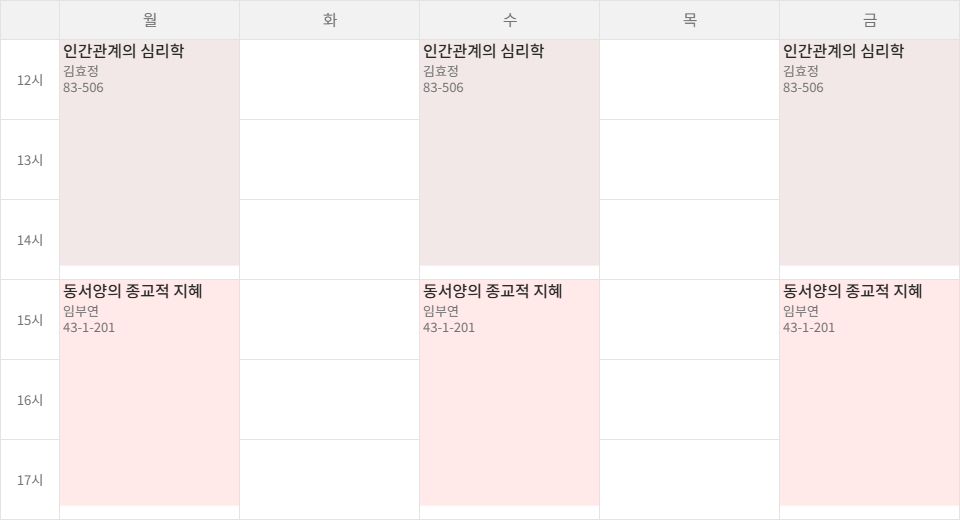
\includegraphics[height=0.72\textheight,width=\linewidth,keepaspectratio]{2026Summer.png}\\[-0.2em]
    {\small 2026 Summer}
  \end{column}
\end{columns}
\end{frame}

\begin{frame}{Mathematics is the foundation of all sciences}
\begin{mainitemize}
  \item 수학은 모든 학문의 기반이다.
  \item 수학을 잘하면 거의 모든 학문을 할 수 있다.
  \item 수학자에게 경제학을 가르칠 순 있지만, 경제학자에게 수학을 가르칠 순 없다.
\end{mainitemize}
\end{frame}

\begin{frame}{Career Path}
\begin{columns}[T,totalwidth=\textwidth]
  \begin{column}{0.48\textwidth}
    \begin{block}{수학과 대학원}
    교수\\연구원\\그 외
    \end{block}
  \end{column}
  \begin{column}{0.48\textwidth}
    \begin{block}{타학과 대학원}
    \vspace{1.8em}
    \end{block}
    \begin{block}{학부 졸업 후 바로 취업}
    \vspace{1.8em}
    \end{block}
  \end{column}
\end{columns}
\end{frame}

\begin{frame}{경희 제74집 합격수기}
\begin{mainitemize}
  \item 수시로 대학을 가자.
  \item 학교 선생님 말씀을 잘 듣자.
  \item 학원에 매몰되지 말자.
  \item 실제로 집중하는 시간이 중요하다.
  \item 쉬는 것도 용기이다.
  \item 특립독행의 길을 걷자.
\end{mainitemize}
\end{frame}

\begin{frame}{수시}
\begin{mainitemize}
  \item 수시로 대학을 가자.
  \item 메디컬이나 서울대를 가려면 내신이 최우선이다.
  \item 포스텍, 카이스트, 고려대, 연세대를 가려면 생기부를 잘 챙기자.
\end{mainitemize}
\end{frame}

\begin{frame}{수시 - 내신}
\begin{mainitemize}
  \item 내신의 출제자는 생각보다 가까이에 있다.
  \item 암기는 모든 학문의 기본이다.
  \item 친구들과 힘을 합치자.
\end{mainitemize}
\end{frame}

\begin{frame}{수시 - 생기부}
\begin{mainitemize}
  \item 본인의 이야기를 담자.
  \item 스토리라인을 구성하자.
  \item 반드시 ‘직접’ 작성하자.
  \item 무작정 어려운 것보다 본인만의 것, 의도가 담긴 것, 특색 있는 것이 중요하다.
\end{mainitemize}
\end{frame}

\begin{frame}{ChatGPT, Gemini, Claude}
\begin{mainitemize}
  \item 생기부 쓸 때 과도하게 사용하지 말자.
  \item 모르는 것을 물어보는 것은 매우 좋으나, 멋있어 보이려고, 수준 높아 보이려고 이해하지도 못한 내용을 생기부에 담으려고 하지 말자.
  \item 교수님들은 생각보다 많이 전문적이시다.
\end{mainitemize}
\end{frame}

\begin{frame}{수시 - 면접}
\begin{mainitemize}
  \item Thinking Process matters.
  \item 본인만의 언어로 설명하는 연습을 하자.
\end{mainitemize}
\end{frame}

\begin{frame}{정시}
\begin{mainitemize}
  \item 수시로 대학을 가라.
  \item 내신 공부가 결국 수능 공부로 이어진다.
  \item 본인의 길을 걷자.
  \item 시간은 많다. Slow and Steady Wins the Race.
  \item 기출문제를 열심히 풀자. \& 수능특강, 수능완성을 풀자.
  \item 27수능이라면 큐레이션에 집중하고, 28수능이라면 기본으로 돌아가자.
\end{mainitemize}
\end{frame}

\begin{frame}{정시 - 국어}
\begin{mainitemize}
  \item 기출문제를 열심히 풀자.
  \item 지문에 집중하자.
  \item 정신을 붙잡는 연습을 하자.
  \item 수준 높은 글을 여러 번 반복해서 읽는 것이 실력 향상의 비결이다.
\end{mainitemize}
\end{frame}

\begin{frame}{정시 - 수학}
\begin{mainitemize}
  \item 기출문제를 열심히 풀자.
  \item 아이디어를 정리하자.
  \item 쉬운 문제는 ‘빨리’ 푸는 것이 중요하다.
  \item 문제의 겉모습에 겁먹지 말자.
  \item 어려운 문제에 도전하는 자와 도전하지 않는 자는 근본적으로 메꿀 수 없는 차이가 난다.
\end{mainitemize}
\end{frame}

\begin{frame}{정시 - 과학}
\begin{mainitemize}
  \item 통합과학은 저도 잘 모릅니당\ldots
  \item 만약 기조가 유지된다면, ‘반응 속도’가 핵심이다.
  \item 사전에 최대한 다양한 문제 상황을 접해봐야 한다.
\end{mainitemize}
\end{frame}

\begin{frame}{FAQ}
\begin{mainitemize}
  \item 포항 너무 멀지 않나요?
  \item 포항 너무 시골 아닌가요?
  \item 서울 자주 오나요?
  \item 학교 성비가 어떻게 되나요?
  \item 수학과에는 남자만 있나요?
  \item 연애하기 어렵나요?
\end{mainitemize}
\end{frame}

\begin{frame}{Live Q\&A}
\vfill
\begin{center}
\begin{tabular}{cccc}
{\Large 발표자} & {\Large 포스텍} & {\Large 수학과} & {\Large 입시}
\end{tabular}
\end{center}
\vfill
\end{frame}

\begin{frame}{Closing Remarks}
\vfill
\begin{center}
{\Large Perfection takes Time}\\[1.2em]
Jungwoo Kim\\
Department of Mathematics, POSTECH
\end{center}
\vfill
\end{frame}

\end{document}
